\chapter{MEG source localisation\label{Chap:data:sloc}}

\section{Overview}
In this section we will generate some simulated data to show how the inversion algorithms compare when the ground-truth is known. 

\section{Simulation}
The code used to generate the simulated data is called \texttt{simmegdip\_for\_faces.m} and is located in the \texttt{example\_scripts} directory. The simulation code takes the experimental setup: sensor locations, triggers, head model etc from the SPM M/EEG dataset\footnote{Multimodal face-evoked dataset: \url{http://www.fil.ion.ucl.ac.uk/spm/data/mmfaces/}}:

\begin{verbatim}
cdbespm8_SPM_CTF_MEG_example_faces1_3D.mat
cdbespm8_SPM_CTF_MEG_example_faces1_3D.dat
\end{verbatim}

you created in chapter \ref{Chap:data:multimodal} and replaces the channel data with simulated data. It also forces the head model to be single-sphere.
You can manipulate this code to change the number or locations of the simulated dipoles by changing

\begin{verbatim}
dipolepositions=[ 52, -29, 13; -52, -29, 13]; % in mni space
\end{verbatim}
or modify the signal vector in anyway to change the time series being simulated. At the simplest level, the matrices \textit{dipamp} and \textit{dipfreq} define how each source behaves during a given condition. 

\begin{verbatim}
% cond 1 cond 2
dipamp=	  [1 		0;...     % dip 1
           1 		0].*1e-1; % dip 2 
dipfreq =	[10 		10;... 	% dip 1
         	20 		20];      % dip 2
\end{verbatim}

That is, the two dipoles are currently set to be on (at 10 and 20Hz) during the faces condition and off during the amplitude condition.

You can run the script to create a new or modified dataset each time. If you run it with no changes, it will generate the dataset:
\\
\texttt{simdata\_aud1020Hz.mat}
\\
This file has dipoles at [52, -29, 13] and  [-52, -29, 13] in  in MNI space. The dipoles are energized at 10Hz and 20Hz from 0.1 to 0.4 seconds (Figure~\ref{meg_sloc:fig:1}). In each epoch the activation profile is identical, the channel data will be slightly different due to the white noise added.

\begin{figure}
\begin{center}
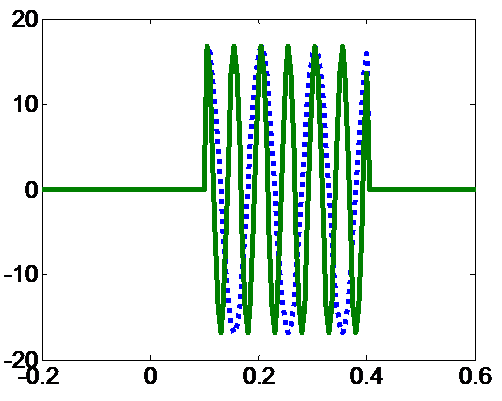
\includegraphics[width=100mm]{meg_sloc/slide1}
\caption{\em Simulated source data \label{meg_sloc:fig:1}}
\end{center}
\end{figure}


\section{Imaging solutions for evoked or induced responses}

On the main menu Click \texttt{3D Source Reconstruction}. Press \texttt{Load}. Select the unaveraged file \texttt{simdata\_aud1020Hz.mat}

Moving left to right along the bottom panel you will notice that all of the buttons (MRI, Co-register, Forward Model) are active. This means that the preprocessing stages have already been carried out on these data (see multi-modal evoked responses chapter).

\subsection{IID (minimum norm)}
We will start off with the traditional minimum norm solution. This starts by assuming that all source elements contribute something to the measured data. The constraint is that the total power (in the sources) should be minimised.
Press \texttt{Invert}. Under reconstruction method press \texttt{Imaging}. For \texttt{All conditions or trials} press \texttt{Yes}. For model press \texttt{Custom}. Model inversion \texttt{IID}. Under Time-window ``0 600''. For \texttt{PST Hanning} select \texttt{Yes}. For High-pass (Hz) select \texttt{1} for Low-pass (Hz) select \texttt{48}. Under \texttt{Restrict solutions} select \texttt{No}. 

\begin{figure}
\begin{center}
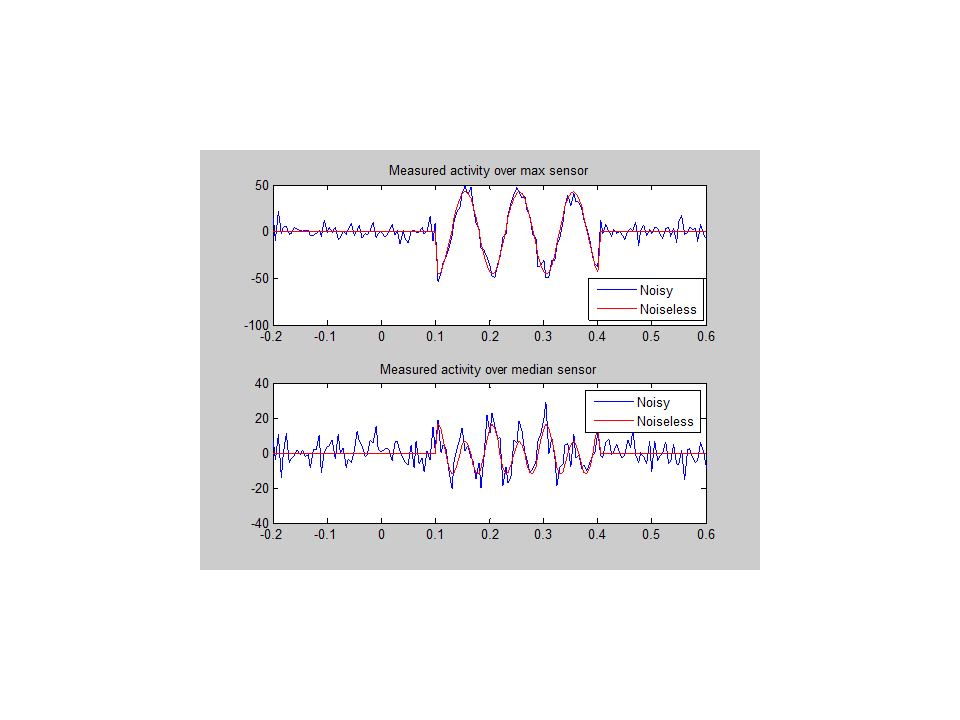
\includegraphics[width=100mm]{meg_sloc/slide2}
\caption{\em IID imaging source reconstruction \label{meg_sloc:fig:2}}
\end{center}
\end{figure}

 
It appears (\ref{meg_sloc:fig:2}) that the minimum norm solution has reconstructed only one of the sources. Note, however, the location of the dotted line in the upper time-series window. The source amplitude reconstruction is based on the location of this line (and conversely the time series shown taken from the maximum image voxel). In the \texttt{ms or mm} box fill in ``205'' then press \texttt{mip}. You should now see that the minimum norm solution is indeed bilateral, although rather diffuse (Figure~\ref{meg_sloc:fig:3}).  Note the log-evidence 8203626.

\begin{figure}
\begin{center}
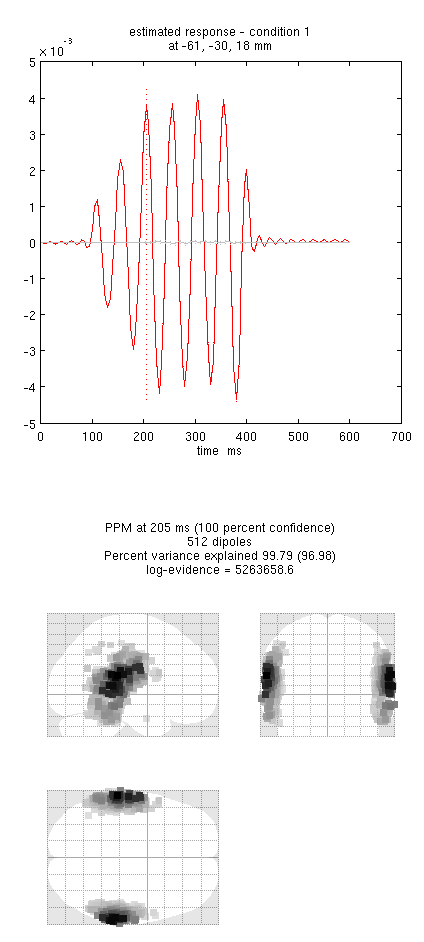
\includegraphics[width=100mm]{meg_sloc/slide3}
\caption{\em IID imaging source reconstruction at 205ms \label{meg_sloc:fig:3}}
\end{center}
\end{figure}

The grey line in the time-series plot shows the amplitude of this voxel in the other ('scrambled') condition. To toggle between the conditions being viewed you can press the \texttt{condition 1/2} button.
Often we will interested in the difference between conditions over a specific time-frequency window, rather than at a single latency. Press the \texttt{Window} button. At the \texttt{Time window (ms)} prompt type ``0 600''. For the \texttt{Frequency [band] of interest (Hz)} type ``1 40''. For \texttt{Power} select \texttt{induced} (although for these data \texttt{evoked} will work just as well). You will now see a glass brain showing a power plot for the current condition. You can convert this image and the corresponding image from the other condition into a volume by pressing \texttt{Image} (Figure~\ref{meg_sloc:fig:4}).

\begin{figure}
\begin{center}
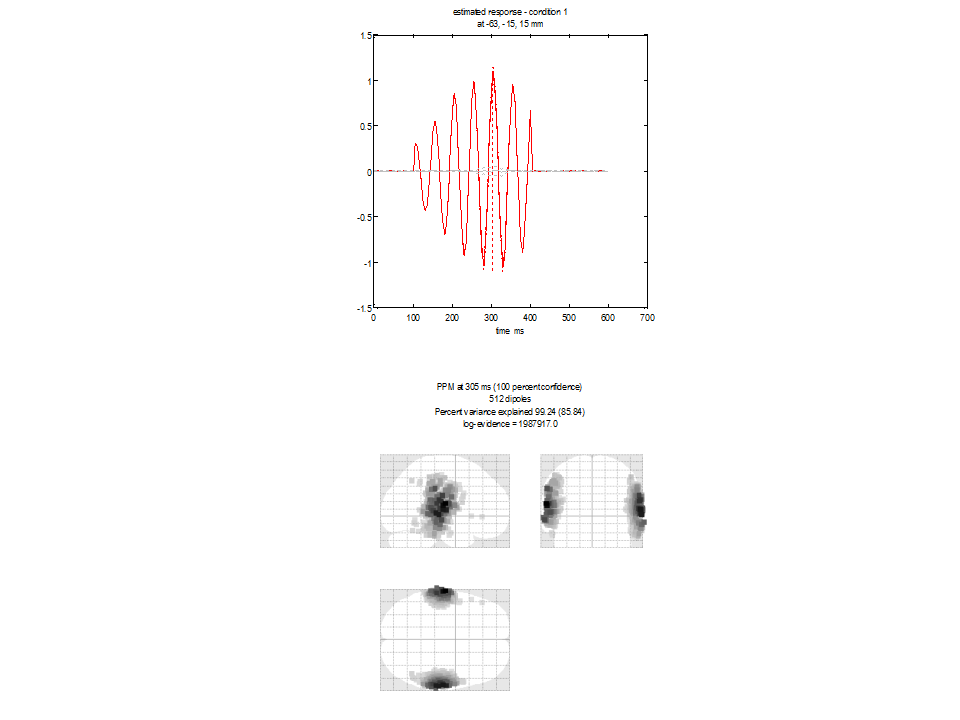
\includegraphics[width=100mm]{meg_sloc/slide4}
\caption{\em Exported functional image from IID source reconstruction overlayed on the template structural image.\label{meg_sloc:fig:4}}
\end{center}
\end{figure}

\subsection{Smooth priors (COH}
The COH option allows the mixture of two possible source covariance matrices: the minimum norm prior above and a much smoother source covariance matrix in which adjacent sources are correlated (over the scale of a few mm). Press \texttt{Invert}. Under reconstruction method press \texttt{Imaging}. For \texttt{All conditions or trials} press \texttt{Yes}. For model press \texttt{Custom}. Model inversion \texttt{COH}. Under Time-window ``0-600''. For \texttt{PST Hanning} select \texttt{Yes}. For High-pass (Hz) select \texttt{1} for Low-pass (Hz) select \texttt{48}. Under \texttt{Restrict solutions} select \texttt{No}.   You will see a plot similar to Figure~\ref{meg_sloc:fig:5} appear. The lower panel shows the glass brain in which bilateral sources are apparent. The upper panel shows the time-series of the source with the largest amplitude. In this case the peak activation is identified at location 59,-32 13. The 10Hz time-course (associated with this source) is also clearly visible in the top panel.  Log evidence is 8211210.

\begin{figure}
\begin{center}
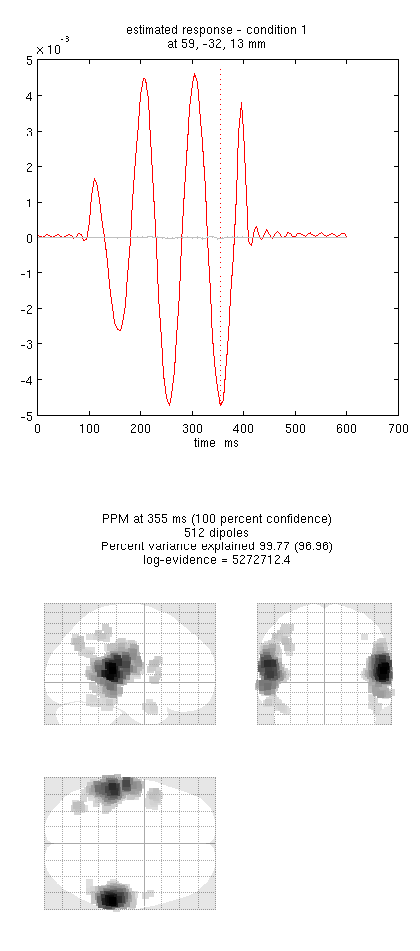
\includegraphics[width=100mm]{meg_sloc/slide5}
\caption{\em COH imaging source reconstruction.\label{meg_sloc:fig:5}}
\end{center}
\end{figure}

\subsection{ARD}
ARD works by creating a basis set of many possible source configurations (e.g. many single sources and left-right symmetric correlated sources) or components. It then works through to eliminate those components which contribute the least (to the model evidence).
Press \texttt{Invert}. Under reconstruction method press \texttt{Imaging}. For \texttt{All conditions or trials} press \texttt{Yes}. For model press \texttt{Custom}. Model inversion \texttt{ARD}. Under Time-window ``0-600''. For \texttt{PST Hanning} select \texttt{Yes}. For \texttt{High-pass (Hz)} select ``1'' for \texttt{Low-pass (Hz)} select ``48''. Under \texttt{Restrict solutions} select \texttt{No}.  In Figure~\ref{meg_sloc:fig:6} the lower panel shows the glass brain in which bilateral sources are apparent and more focal than previously observed. This becomes more evident if you now work through to produce a contrast. Press the \texttt{Window}, \texttt{Time window (ms)} prompt type ``0 600''. \texttt{Frequency [band] of interest (Hz)} type ``1 40'', for \texttt{Power} select \texttt{induced}. Then press \texttt{Image} to see the result overlaid on an MNI brain (Figure~\ref{meg_sloc:fig:7}). Note the evidence 8379513.

\begin{figure}
\begin{center}
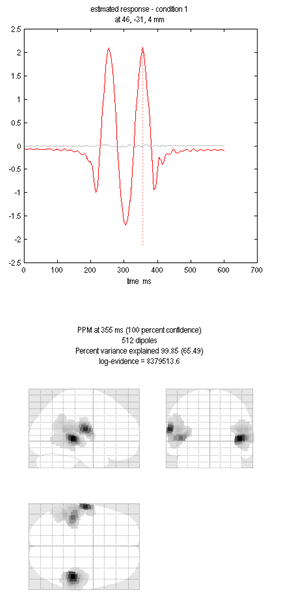
\includegraphics[width=100mm]{meg_sloc/slide6}
\caption{\em ARD imaging source reconstruction.\label{meg_sloc:fig:6}}
\end{center}
\end{figure}


We could now make a volume to compare with the minimum norm solution (Figure~\ref{meg_sloc:fig:4}) \footnote{Note that you need to copy the previously generated image files to a different directory to prevent them from being overwritten}. Press the \texttt{Window} button. At the \texttt{Time window (ms)} prompt type ``0 600''. For the \texttt{Frequency [band] of interest (Hz)} type ``1 40''. For \texttt{Power} select \texttt{induced} (although for these data \texttt{evoked} will work just as well). You will now see a glass brain showing a difference in power plot between the two conditions. You can convert this into a volume by pressing \texttt{Image} (Figure~\ref{meg_sloc:fig:7}).

\begin{figure}
\begin{center}
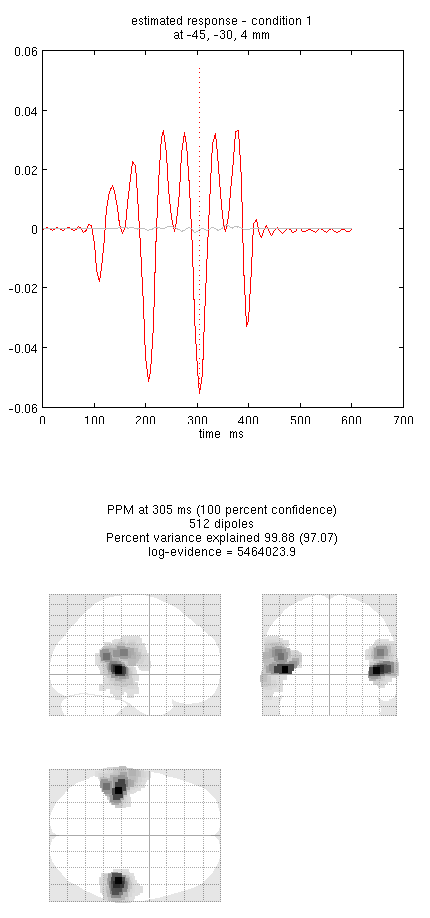
\includegraphics[width=100mm]{meg_sloc/slide7}
\caption{\em Exported functional image from ARD source reconstruction overlayed on the template structural image.\label{meg_sloc:fig:7}}
\end{center}
\end{figure}


\subsection{Greedy Search (GS)}
In contrast to ARD, the greedy search routine builds up successive combinations of source configurations until the model evidence can no longer be improved.
Press \texttt{Invert}. Under reconstruction method press \texttt{Imaging}. For \texttt{All conditions or trials} press \texttt{Yes}. For model press \texttt{Custom}. Model inversion \texttt{GS}. Under Time-window ``0-600''. For \texttt{PST Hanning} select \texttt{Yes}. \texttt{For High-pass (Hz)} select \texttt{1} for \texttt{Low-pass (Hz)} select ``48''. Under \texttt{Restrict solutions} select \texttt{No}.  Note again the more focal sources (Figure~\ref{meg_sloc:fig:8}) as compared to the minimum norm solution; although the time-series estimation seems to have suffered. Note the evidence 8374355.

\begin{figure}
\begin{center}
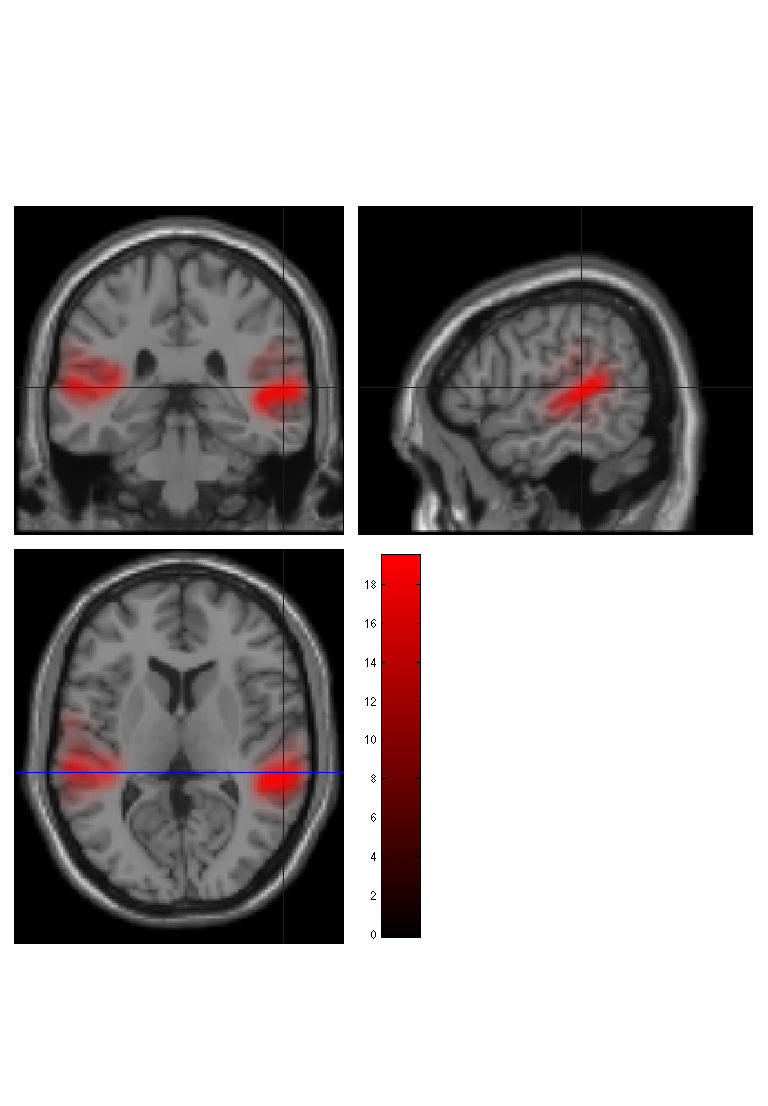
\includegraphics[width=100mm]{meg_sloc/slide8}
\caption{\em GS imaging source reconstruction.\label{meg_sloc:fig:8}}
\end{center}
\end{figure}

\subsection{Multiple Sparse Priors (Standard)}
The standard button is simply the use of a greedy search using the whole time window available in a band of 2-128Hz. following default options: Greedy Search, all time, hanning windowed, filter 2-128Hz.

\subsection{Model comparison}.
As we tested all the above models on the same data we can make a model comparison. Figure~\ref{meg_sloc:fig:9} shows that the ARD model is marginally superior to the GS and both of these improve upon IID and COH solutions.

\begin{figure}
\begin{center}
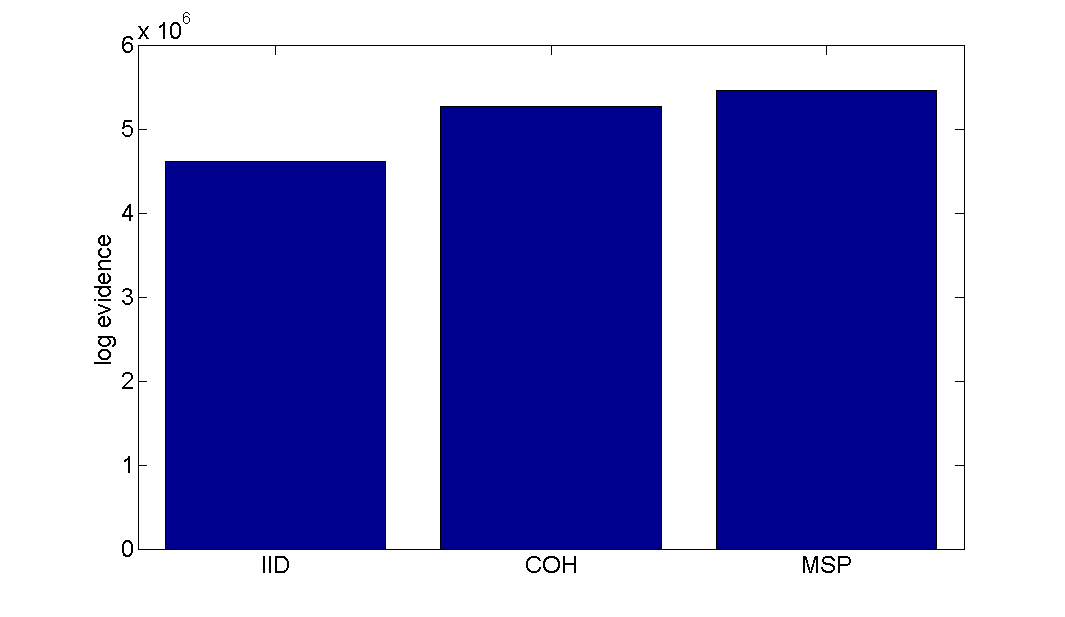
\includegraphics[width=100mm]{meg_sloc/slide9}
\caption{\em Bayesian model evidence for different prior specifications.\label{meg_sloc:fig:9}}
\end{center}
\end{figure}


\section{Beamformer analysis}
In this final stage we will look for differences between the conditions using the linear constrained minimum variance beamformer. The main assumption in beamformer imaging is that there is no covariance between the underlying sources. That is, the prior source covariance matrix is a diagonal, the elements of which can be directly estimated from the sample covariance (Hillebrand et al 2005).
The current beamformer implementations differ from the above in that they test points throughout the source space (i.e. not just on the cortical surface) and do not provide model evidence. At present therefore the beamformer routines sit apart from the other imaging reconstruction methods, but rely on the same coregistration and forward model selection.

\subsection{LCMV beamformer}
On the main SPM menu select the Toolbox pull-down menu. Under \texttt{Beamforming} select \texttt{Volumetric LCMV beamformer}.
Select file \texttt{sim\_data\_aud1020Hz.mat}.
The first menu will ask you to select the active condition. Select 'faces' and click \texttt{OK}. You will then be asked at what time the condition 'faces' begins.  At \texttt{Offset (ms) from faces}, type 0. At the duration prompt type 600. i.e. we are using the same 0-600ms window as before. At the baseline condition prompt select 'scrambled'. \texttt{Offset ms from scrambled} should be set to 0ms also. We will be comparing the same time window 0-600ms across epochs labelled either scrambled, or faces. At the number of frequency bands prompt type ``2''. The more frequency bands one computes at this stage the smaller the overhead in time. For the first band type ``15 25'', for the second try ``1 48''. For \texttt{gridstep} type ``10'' mm (number of voxels hence speed decreases by a factor of 8 each time this is halved). Leave regularization at 0. Select \texttt{yes} for preview results.
As you selected preview you will see an image similar to Figure~\ref{meg_sloc:fig:10}, in which we restricted our analyses to the frequency band around one source. This is a t-statistic image showing the difference between the two conditions (note in this image left is on right). You can navigate through the image using the mouse and need to press  \texttt{q} to leave the window. The second figure produced Figure~\ref{meg_sloc:fig:11} should be comparable with the previous time-window analyses on the 1-48Hz band. 

\begin{figure}
\begin{center}
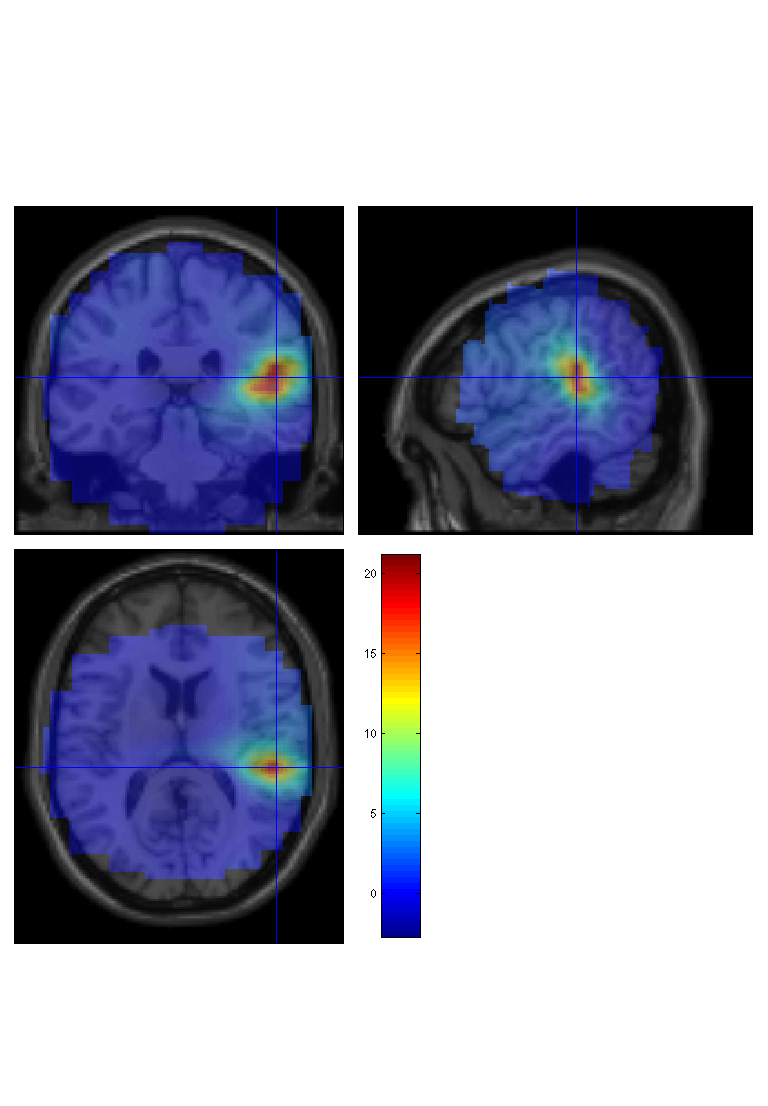
\includegraphics[width=100mm]{meg_sloc/slide10}
\caption{\em LCMV beamformer results for 15-25Hz.\label{meg_sloc:fig:10}}
\end{center}
\end{figure}

\begin{figure}
\begin{center}
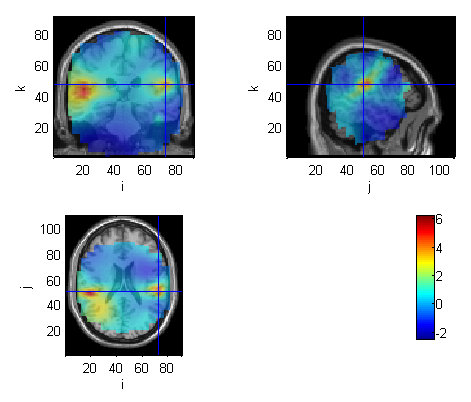
\includegraphics[width=100mm]{meg_sloc/slide11}
\caption{\em LCMV beamformer results for 1-48Hz.\label{meg_sloc:fig:11}}
\end{center}
\end{figure}

Now to compare the beamformer images with some of our other reconstructions:

You will find the volumetric images within the sub-directory \texttt{''tstatBf\_images}. You can use the \texttt{''checkReg} button to compare these images with other volumes (produced above using the \texttt{Window''/``Image} options. In Figure~\ref{meg_sloc:fig:12} the ARD and beamformer 0-600ms, 1-48Hz contrasts are shown alongside an anatomical image from the spm/templates directory.

\begin{figure}
\begin{center}
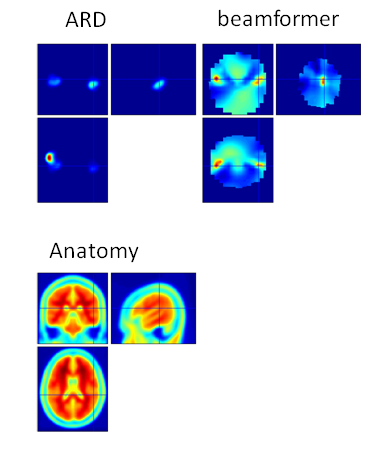
\includegraphics[width=100mm]{meg_sloc/slide12}
\caption{\em Comparison of ARD and LCMV beamformer results.\label{meg_sloc:fig:12}}
\end{center}
\end{figure}

\subsection{DICS beamformer}
In \texttt{Beamforming} select \texttt{Fieldtrip DICS beamformer}. For a change we will simply test the faces condition across two different time windows. Under \texttt{Select conditions} select 'faces'. For \texttt{Frequency range} choose ``1 48''. For \texttt{Number of time windows} enter ``2''. For the first time window enter ``-0.2 0'' (i.e. baseline). For the second enter ``0.1 0.3''. Change the contrast vector to ``-1 1'' i.e. it will subtract the first condition (baseline) from the second. For \texttt{regularization'} select ``0'', for \texttt{preview results} select \texttt{yes}. You will see something like Figure~\ref{meg_sloc:fig:13}. Note that this is not a statistical image, but simply the difference of the power in the pre- and post-stimulus faces condition.  As source estimates tend to be large near the centre of the head (as the lead fields are small) these large differences remain in the final image. If you do proper statistical test over trials the activations in the centre of the head should not appear because of their high variability.

\begin{figure}
\begin{center}
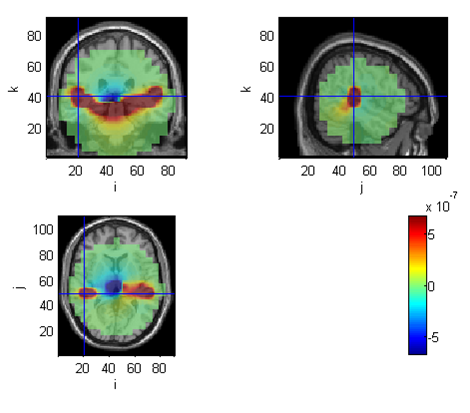
\includegraphics[width=100mm]{meg_sloc/slide13}
\caption{\em DICS beamformer results.\label{meg_sloc:fig:13}}
\end{center}
\end{figure}

\section{Dipole fitting to the average}

Up until this point the analysis we have used could have been applied to either induced or evoked changes in electrical activity. The only difference being that it would not have made much sense to look at the MSPs for specific time-instants in the induced case and we would have proceeded directly to look for changes in a time-frequency window. To examine the dipole fit routine we will however concentrate on the averaged data file which will contain only evoked changes.

\subsection{Load/preview the data}

In the main menu click on the drop-down \texttt{Display} menu. Select \texttt{M/EEG}. For the dipole fitting we are going to use averaged MEG data, this is prefixed with an ``m'' in SPM. You can generate this file by averaging the epoched file that we have used until now. Select the file:

\begin{verbatim}
msimdata_aud1020Hz.mat
\end{verbatim}

You will now see the simulated data. You will be looking at the ``Trial 1 (..) Faces'' trial,  but if you switch (top-right menu) to ``Trial 2 (..) scrambled'' you will see that our simulated sources are not active during this condition.  If you now click on the field map button you will see a cursor on the time-series plot and a field map for this time instant as in figure 3. Use the slider at the bottom of the field map to vary the time instant plotted. At 205ms (Figure~\ref{meg_sloc:fig:14}A) you will notice that there are clearly two dipolar patterns, whereas at 235ms (Figure~\ref{meg_sloc:fig:14}B) there is only one.
We will now move on to explore Bayesian dipole fitting to these two time instants.

\begin{figure}
\begin{center}
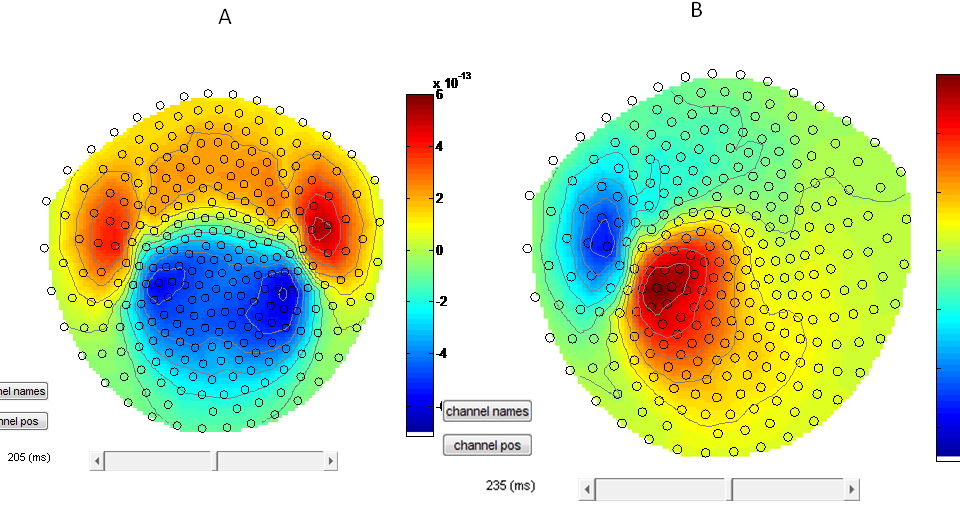
\includegraphics[width=100mm]{meg_sloc/slide14}
\caption{\em Scalp maps for averaged simulated data.\label{meg_sloc:fig:14}}
\end{center}
\end{figure}

\subsection{Inversion}
In the main menu window, select \texttt{3D Source Reconstruction}. Click \texttt{Load} and select the averaged simulated dataset above.
Proceed by pressing the \texttt{Invert} button. Select the \texttt{VB-ECD} button.

\subsubsection{Fitting a single dipole with no priors}
At the \texttt{time\_bin or average\_win} prompt enter ``235''. For \texttt{Trial type number} choose ``1'' (we want to model the faces data). At the \texttt{Add dipoles to model} click \texttt{Single}. For \texttt{location prior} click \texttt{Non-info}. For \texttt{Moment prior} click \texttt{Non-info}. At the \texttt{Add dipoles to 1 or stop?} prompt click \texttt{stop}. Leave the default number of iterations at ``10''.
You will see the 10 successive fits of the same data using a random starting location and moment. At each fit maps of the predicted and simulated data along with free-energy values and percent variance explained are shown. The final plot will be similar to Figure~\ref{meg_sloc:fig:15} where the model (i.e. dipole) which maximised the evidence (the best iteration is shown with a red dot) is displayed. Note down the model evidence (in this case -4.3). The Bayesian dipole fit algorithm will be most useful when one has some prior knowledge of the sources (such as location, orientation or symmetry). Typical dipole fit algorithms fit 3 location parameters per dipole and then estimate the moment through a pseudo-inverse. The VB-ECD algorithm however fits 6 parameters per dipole as the moments are also allowed prior values. That is, if you have no prior knowledge then the Bayesian method will be generally less robust than such fitting methods (as more parameters are being fit). However it is when prior knowledge is supplied that the Bayesian methods become optimal.

\begin{figure}
\begin{center}
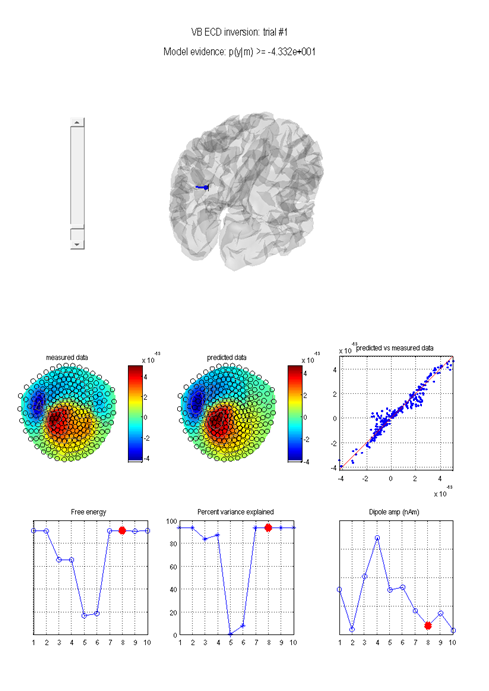
\includegraphics[width=140mm]{meg_sloc/slide15}
\caption{\em Results of fitting a single dipole with noninformative priors.\label{meg_sloc:fig:15}}
\end{center}
\end{figure}


\subsubsection{Fitting a single dipole with reasonable and unreasonable priors}
We will now provide some prior knowledge to the dipole fit perhaps led by the literature or a particular hypothesis. In this case we know the answer, but let us specify a location a couple of cm from where we know the source to be (at -52,-29,13mm) and try the fit again.
At the  \texttt{time\_bin or average\_win} prompt enter ``235''. For  \texttt{Trial type number} choose ``1'' (we want to model the faces data). At the  \texttt{Add dipoles to model} click  \texttt{Single}. For  \texttt{location prior} click  \texttt{Informative}. For the location enter ``-62 -20 10''. For prior location variance leave at ``100 100 100'' mm$^2$. This means that we are not sure about the source location to better than 10mm in each dimension. For  \texttt{Moment prior} click  \texttt{Non-info}. At the  \texttt{Add dipoles to 1 or stop?} prompt click  \texttt{stop}. Leave the default number of iterations at ``10''. Again you will get a final fit location and model evidence (-3.8), which should have improved (be more positive) on the evidence above. 
Now go through exactly the same procedure as above but for the prior location enter ``+62 -20 10'', i.e. on the wrong side of the head. You will note that the algorithm finds the correct location but the evidence for this model (with the incorrect prior) is much lower (-8.4). You could also try to fit a symmetric pair to this latency dataset (see below), model evidence -150.

\subsubsection{Fitting more dipoles}
We will start by examining the time instant at which we can clearly see a two-dipolar field pattern.
At the \texttt{time\_bin or average\_win} prompt enter ``205''. For \texttt{Trial type number} choose ``1''. At the \texttt{Add dipoles to model} click \texttt{Single}. For \texttt{location prior} click \texttt{Informative}. For the location enter ``62 -20 10''. For prior location variance enter ``400 400 400'' mm$^2$, that is, the prior standard deviation on the dipole location is 20mm in each direction. For \texttt{Moment prior} click \texttt{Non-info}. At the \texttt{Add dipoles to 1 or stop?} prompt click \texttt{Single}. For \texttt{location prior} click \texttt{Informative}. For the location enter ``-62 -20 10''. For prior location variance enter ``400 400 400'' mm$^2$. At the \texttt{Add dipoles to 1 or stop?} prompt click \texttt{stop}. Leave the default number of iterations at ``10''. Note down the final model evidence (570). 

Alternatively we can exploit the fact that we have prior knowledge that the dipoles will be approximately left-right symmetric in location and orientation. At the \texttt{time\_bin or average\_win} prompt enter ``205''.  For \texttt{Trial type number} choose ``1''. At the \texttt{Add dipoles to model} click \texttt{Symmetric Pair}. For \texttt{location prior} click \texttt{Informative}. For the location enter \texttt{62 -20 10}. For prior location variance enter ``400 400 400'' mm$^2$. For \texttt{Moment prior} click \texttt{Non-info}. At the \texttt{Add dipoles to 2 or stop?} prompt click \texttt{stop}. Leave the default number of iterations at ``10''. Note that the final locations are approximately correct, but importantly the model evidence (-9.6) is much lower than previously. Given this information one would accept the two distinct dipole model over the symmetric pair. 

Finally we can take our best model so far, and try adding in an extra source.
At the \texttt{time\_bin or average\_win} prompt enter ``205''. For \texttt{Trial type number} choose ``1''. At the \texttt{Add dipoles to model} click \texttt{Single}. For \texttt{location prior} click \texttt{Informative}. For the location enter ``62 -20 10''. For prior location variance enter ``400 400 400'' mm$^2$, that is, the prior standard deviation on the dipole location is 20mm in each direction. For \texttt{Moment prior} click \texttt{Non-info}. At the \texttt{Add dipoles to 1 or stop?} prompt click \texttt{Single}. For \texttt{location prior} click \texttt{Informative}. For the location enter ``-62 -20 10''. For prior location variance enter ``400 400 400'' mm$^2$. At the \texttt{Add dipoles to 2 or stop?} prompt click \texttt{Single}. We will add an extra dipole that can be anywhere in the head, so for \texttt{Location Prior} click \texttt{Non-info}. For \texttt{Moment Prior} click \texttt{non-info}. At the \texttt{Add dipoles to 2 or stop?} prompt click \texttt{Stop}. Leave the default number of iterations at ``10''. Note down the final model evidence (550). That is, the evidence has now begun to decrease once more suggesting that the two distinct dipole model is the best for these data.

